\documentclass{ctexart}
\usepackage{amssymb,amsfonts,amsmath,amsthm}
%--------
% 设置字体
%--------




%----------
% 版面设置
%----------
%首段缩进
\usepackage{indentfirst}
\setlength{\parindent}{2em}

%行距
\renewcommand{\baselinestretch}{1.5} % 1.5倍行距

%页边距
\usepackage[a4paper]{geometry}
\geometry{verbose,
  tmargin=2cm,% 上边距
  bmargin=2cm,% 下边距
  lmargin=3cm,% 左边距
  rmargin=3cm % 右边距
}


%----------
% 其他宏包
%----------
\usepackage{enumerate}
\usepackage{geometry}
\usepackage{fontspec}
\usepackage{listings}
\usepackage{xcolor}
\usepackage{graphicx}
\usepackage{subfigure}
\usepackage{caption}
\usepackage{pdfpages}%插入PDF
\usepackage{booktabs}
\usepackage{multirow}
\usepackage{siunitx}

\graphicspath{{figures/}{logo/}}%声明图片和logo目录

%-----------
%页眉页脚
%-----------
\usepackage{fancyhdr}
\setlength{\headheight}{14pt}
\pagestyle{fancy}
\lhead{}
\chead{\kaishu SVPWM原理、实现与数学表达}
\rhead{ }
\cfoot{\thepage}


%-----------
%取消Section编号
%-----------
%\setcounter{secnumdepth}{-2}


%-------------
%公式编号加入节section
%-------------
\numberwithin{equation}{section}


%-------------
%new command 公式
%-------------



%-----------
%正文
%-----------


\begin{document}


\title{\heiti SVPWM原理、实现与数学表达}    
\author{\kaishu 李华康 \\huakang.li@outlook.com}  
\date{2020.06}
\maketitle


SVPWM的主要思想是以三相对称正弦波电压供电时三相对称电动机定子理想磁链圆为参考标准,
以三相逆变器不同开关模式作适当的切换,从而形成PWM波,以所形成的实际磁链矢量来追踪其准确磁链圆。
——百度百科(王兆安《电力电子技术基础》)。

电压空间矢量调制SVM的思想源于交流异步电机变频调速。——陈坚《电力电子学》。

作为电气专业的学生,我们很多时候是基于电机来理解空间矢量的。但是,给它过多的物理含义其实并没有意义。空间矢量调制完全可以通过数学的方法来理解。

\section{相量、矢量、时间、空间}
在正式讨论SVPWM之前,我们要明确与辨析一些基本概念的含义,即相量,矢量,时间与空间。

\subsection{相量}
需要说明的是,相量对于分析SVPWM并没有太多帮助,但是明确的区分相量和空间矢量。相量是为了分析正弦稳态电路而人为定义的一个矢量。对于一个正弦稳态的电气信号,它包含三个基本要素,即幅值、频率和初相位。下面以电压信号为例,三相对称电压信号的表达式为

\begin{equation}
  \begin{aligned}
  	&u_A(t) = U_m \sin (\omega t)\\
  	&u_B(t) = U_m \sin (\omega t - 2/3\pi)\\
  	&u_C(t) = U_m \sin (\omega t + 2/3\pi)
  \end{aligned}
\end{equation}
$ u_A $、$ u_B $、$ u_C $的幅值均为$ U_m $,频率均为$ \omega $,而初相位分别为0,-2/3$ \pi $和2/3$ \pi $。所以要区分$ u_A $、$ u_B $、$ u_C $,只需要将它们的初相位单独标识出来即可,也就是说,$ u_A $、$ u_B $、$ u_C $可分别记为$ \angle 0 $、$ \angle -2/3\pi $、$ 2/3\pi $。在同一个电路系统中,往往只有一个频率,但是可能有几个电压,所以在初相位信息的基础上再加上幅值信息,就可以表达出这个系统中的所有电压电流信号了,而这个表示系统就是相量表达。因此$ u_A $、$ u_B $、$ u_C $完整的相量表达就是$ \dot U_A = U_m\angle 0 $、$ \dot U_B = U_m\angle -2/3\pi $、$\dot U_C = U_m2/3\pi $。

但是光表示还是远远不够的,这套表示系统还需要具备可运算的功能才有实际用处。可以很清楚的看到,相量之间的运算其实就是正弦函数之间的运算。正弦函数直接进行运算往往非常麻烦,但是如果能将正弦函数之间的运算转换到更加简单的系统当中去,相量表示法将变得更加有价值。而欧拉公式(式1.2)正是这样一个非常好的连接工具。
\begin{equation}
  Ue^{j(\omega t + \varphi)} = U\cos (\omega t + \varphi) +jU\sin (\omega t + \varphi)
\end{equation}
一个复指数函数的实部或虚部都包含了正弦信号,且稳态正弦信号中角频率固定不变,$Ue^{j\varphi} \to U\sin(wt+\varphi)$ 这个映射保持加法运算,是加法群同构\footnote{何子涵同学指导},因此通过对复指数函数的运算就可以实现对相量的运算。所以$ u_A $、$ u_B $、$ u_C $用带指数函数的相量形式可以写作$ \dot U_A = U_m e^{j0} $、$ \dot U_B = U_m e^{j-2/3\pi} $、$ \dot U_C = U_m e^{j2/3\pi} $。

\subsection{矢量}
又称相量,是一种既有大小又有方向的量。从相量的复指数函数定义可以看出,相量其实就是一种矢量,其大小可以表示电信号的幅值,其方向可以表示电信号的相位信息,并且它的运算遵循平行四边形法则。可以看到相量代表的矢量,有着明确的物理意义。但是SVPWM中的矢量则很大程度上是为了数学上的方便而认为造出来的。

\subsection{空间}
事实上任何矢量都必须存在于某一个空间,相量矢量也是,它的矢量空间就是复平面。所以单说空间矢量其实是意义不明的,在SVPWM中的空间矢量,是人为规定的在某一个特定空间内存在的特定矢量。在叙述这个特定矢量空间之前,让我们先从另一个矢量空间说起,如图\ref{abc-space}左侧所示,并将其记为“ABC空间”。在这个空间中,有ABC三个轴,这三个轴上的基底长度都是1,方向依次增加\ang{120} 。
同时有幅值为1的三相对称正弦信号$u_a$、$u_b$、$u_c$,相位依次滞后\ang{120},如图\ref{abc-space}右侧所示,并将其记为“abc系统”。

将abc系统中$u_a$、$u_b$、$u_c$的大小分别作为ABC空间中A、B、C三个轴上矢量$\vec{x_{a}}$、$\vec{x_{b}}$、$\vec{x_{c}}$的长度大小,并将这三个矢量依据平行四边形法则进行合成得到矢量$\vec{x_F}$。
比如在$ \omega t = \pi /2 $时,$ \vert \vec{x_a} \vert = 1 $,$ \vert \vec{x_b} \vert = 1/2 $,$ \vert \vec{x_c} \vert = 1/2 $,合成相量$  \vec{x_F} $的长度为3/2,而方向与A轴基底方向相同。
类似的,在$ \omega t = \frac{7}{6}\pi $时,$ \vert \vec{x_a} \vert = 1/2 $,$ \vert \vec{x_b} \vert = 1 $,$ \vert \vec{x_c} \vert = 1/2 $,合成相量$  \vec{x_F} $的长度为3/2,而方向与B轴基底方向相同。
在$ \omega t = \frac{11}{6}\pi $时,$ \vert \vec{x_a} \vert = 1/2 $,$ \vert \vec{x_b} \vert = 1/2 $,$ \vert \vec{x_c} \vert = 1 $,合成相量$  \vec{x_F} $的长度为3/2,而方向与C轴基底方向相同。可以发现,合成矢量 $ \vec{x_F} $的长度并没有改变而只是方向发生了变化。事实上,通过数学可以证明,合成矢量 $ \vec{x_F} $是一个长度保持3/2不变且在空间中匀速旋转的矢量,旋转方向为逆时针方向,旋转速度等于abc系统中角频率 $ \omega $。

\begin{figure}[hbtp]
\centering
\begin{minipage}[b]{0.48\linewidth}
\centering
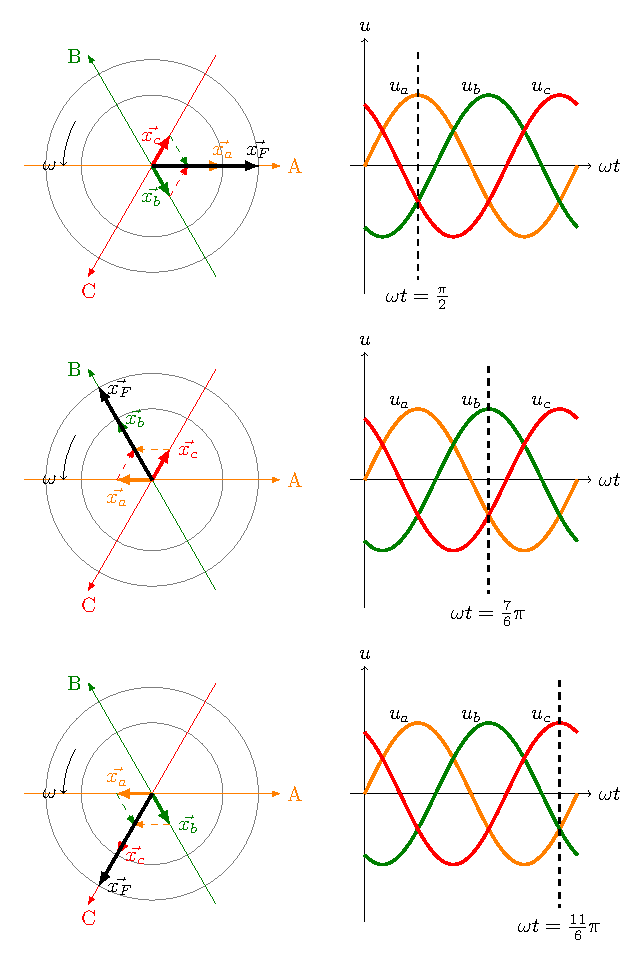
\includegraphics[width = \linewidth]{ABC-vector-space.pdf}
\caption{ABC空间 - abc系统}
\label{abc-space}
\end{minipage}
\hspace{10pt}
\begin{minipage}[b]{0.48\linewidth}
\centering
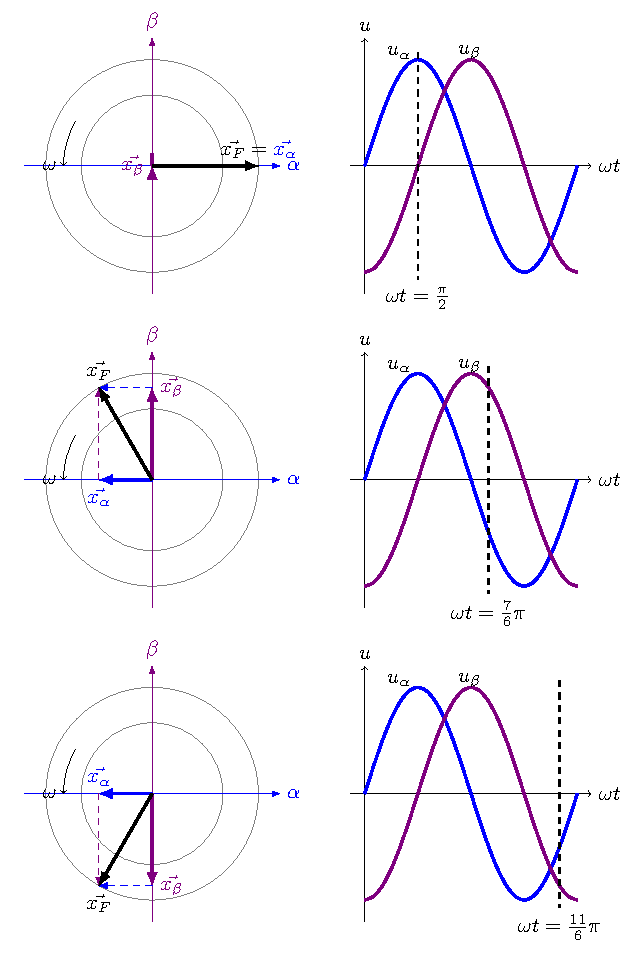
\includegraphics[width = \linewidth]{alpha-beta-space.pdf}
\caption{$\alpha \beta $空间 - $\alpha \beta $系统}
\label{alpha-beta-space}
\end{minipage}
\end{figure}

由以上分析可知,ABC空间中的$ \vec{x_F} $与abc系统二者之间可以通过一套数学公式相互转换。事实上,要合成矢量$ \vec{x_F} $并不需要三个基底,而只需要两个不平行的基底就行。通常情况,可以选择两个正交的基底,如图\ref{alpha-beta-space}左侧所示,为了与之前的三个基底的表达方式进行区别,将其记为“$\alpha \beta$空间”。$\alpha \beta$空间中共有两个轴,基底长度均为3/2,方向上$ \beta $轴比$ \alpha $轴大\ang{90}。设在$\alpha \beta$空间中有与ABC空间中相同的旋转矢量$ \vec{x_F} $,并将这个矢量在$ \alpha $轴和$ \beta $轴上分解为$\vec{x_{\alpha}}$和$\vec{x_{\beta}}$。将$\vec{x_{\alpha}}$和$\vec{x_{\beta}}$的长度大小记为${u_{\alpha}}$和${u_{\beta}}$,画出${u_{\alpha}}$和${u_{\beta}}$随旋转相位$\omega t$的变化关系如图\ref{alpha-beta-space}右侧所示,其中让$\alpha \beta$空间中旋转矢量的初相位与$ABC$空间中旋转矢量的初相位保持一致。将${u_{\alpha}}$和${u_{\beta}}$这样的正交两相正弦信号记为“$\alpha \beta$系统”。这样abc系统就通过空间旋转矢量与$\alpha \beta$系统建立了联系,可以说这两个系统其实表达了相同的信息。为什么一个三相信号可以转换为一个两相信号了,这是因为对称的三相信号彼此并不完全独立,它们在任何时候的和都为0,因此只需要两相信号就可以完整地表达三相信息。

abc系统向$\alpha \beta$系统的变换就是所谓的Clarke变换,见式\ref{clarke transformation},相应地,$\alpha \beta$系统向abc系统的变换就是Clarke反变换,见式\ref{inverse clarke transformation}。在上面的分析中我们让旋转矢量的长度相等,得到${u_{\alpha}}$和${u_{\beta}}$的幅值是3/2,通过调整Clarke变换与反变换中的系数$m$和$m'$,可以调整abc系统和$\alpha \beta$系统中的幅值大小。$m=2/3$和$m'=1$时,abc系统和$\alpha \beta$系统中的幅值大小相等;$m=\sqrt{2/3}$和$m'=\sqrt{2/3}$时,abc系统和$\alpha \beta$系统中的功率大小相等。
\begin{align}
  \text{Clarke Transformation:}
  &\begin{bmatrix}
    u_{\alpha}\\
    u_{\beta}
  \end{bmatrix}
  =
  m
  \begin{bmatrix}
    1 & -\frac{1}{2} & -\frac{1}{2}\\
    0 & \frac{\sqrt{3}}{2} & -\frac{\sqrt{3}}{2}
  \end{bmatrix}
  \begin{bmatrix}
    u_a\\
    u_b\\
    u_c
  \end{bmatrix}
  \label{clarke transformation}
  \\
  \text{Inverse Clarke Transformation:}
  &\begin{bmatrix}
    u_a\\
    u_b\\
    u_c
  \end{bmatrix}
  =
  m'
  \begin{bmatrix}
    1 & 0\\
    -\frac{1}{2} & \frac{\sqrt{3}}{2}\\
    -\frac{1}{2} & -\frac{\sqrt{3}}{2}
  \end{bmatrix}
  \begin{bmatrix}
    u_{\alpha}\\
    u_{\beta}
  \end{bmatrix}
  \label{inverse clarke transformation}
\end{align}

在之前我们借助旋转矢量讲述了这个变换,其实这个旋转矢量在Clarke变换的数学解释中完全是多余的,但是空间旋转矢量对于理解与应用Clarke变换非常有帮助。

\subsection{时间}
在对正弦稳态信号的分析中,时间信息其实是和频率信息高度捆绑在一起的,在相量系统中,时间信号伴随着频率系统一起被省略。而在空间矢量系统中,频率和时间则可以被拿出来讨论,但是这里的频率并不是正弦稳态信号中的频率,而是空间矢量旋转的角速度。严格来说,只有稳定的正弦信号才能有频率这一概念,如果旋转矢量的角速度发生变化,那么它不再对应一个稳定的三相对称信号,但是在瞬时,我们可以近似认为旋转矢量角速度不变,从而对应一个三相对称稳态正弦信号,虽然它在物理上并不存在,但是这将有助于我们跟踪和控制三相交流系统的频率。在这种定义下,频率可认为是电信号相位$\theta$对时间的导数,即
\begin{equation}
  \omega = \frac{d\theta}{dt}
\end{equation}

下面将给出一个实例具体阐述。如现在希望得到一个幅值和频率都从0开始随时间线性增加,直至0.2$s$后达到期待幅值100A和频率60Hz的三相交流电流。从0-0.2$s$的整体来看,这个三相系统都是不稳定的,频率和幅值也就无从谈起,但是如果我们认为它在瞬时“稳定”,那么问题就可以得到解决。因此
\begin{equation}
  \omega = \frac{d\theta}{dt} = 120\pi kt
\end{equation}
式中,$ k = 1/0.2 = 5 $。假定参考信号的初相位为0,则
\begin{equation}
  \theta = \int_0^{t} \omega dt = 60\pi kt^2
\end{equation}
因此三相交流电流的数学表达式为
\begin{equation}
  \begin{aligned}
  	&i_a = 100kt\sin (60\pi kt^2 )\\
  	&i_a = 100kt\sin (60\pi kt^2 -\frac{2}{3}\pi )\\
  	&i_a = 100kt\sin (60\pi kt^2 + \frac{2}{3}\pi )
  \end{aligned}
\end{equation}
0.2$ s $之后,各相电流维持为60Hz和100$ A $的正弦波,画出0-0.25$ s $三相电流波形,如图\ref{kw-kA-sine-wave}所示。

\begin{figure}[hbt]
  \centering
  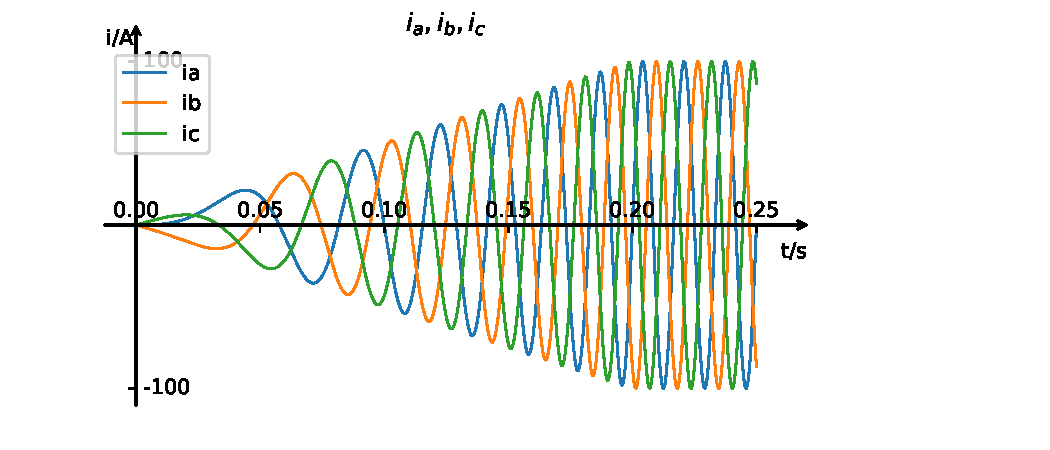
\includegraphics[width = .8\linewidth ]{sin_wave_kA_kw}
  \caption{0-0.25$ s $三相电流信号波形}
  \label{kw-kA-sine-wave}
\end{figure}

\section{SVPWM原理}
SVPWM在最早出现时,与电机的旋转磁链有关,但是后来SVPWM也广泛用于其他三相电力电子变换和控制之中。这是因为任何三相对称正弦系统都能通过坐标变换的数学方式得到类似旋转磁链的空间旋转矢量。通过控制电机的磁链追踪理想磁链圆可以达到控制电机的目的,同样的,通过控制电力电子变换器的三相信号经坐标变换产生的空间矢量追踪理想矢量圆,也可以达到控制电力电子变换器的目的。

\begin{figure}[hbtp]
  \centering
  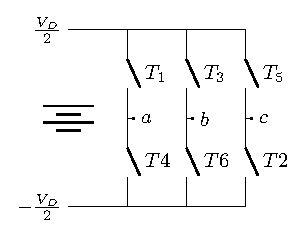
\includegraphics[width = .5\linewidth ]{three-phase-converter.pdf}
  \caption{三相两电平电压型逆变器电路}
  \label{three-phase-converter}
\end{figure}  

以三相两电平电压型逆变器为例。如图\ref{three-phase-converter}所示,逆变器一共有3个桥臂,分别将其记为a桥臂、b桥臂和c桥臂,每个桥臂同时只允许一个开关管导通,因此总共就有8种开关状态组合。将各相桥臂的上管导通下管关断记为1,相反将桥臂的上管关断下管导通记为0。以a-b-c的顺序依次记下三个桥臂的开关状态,即这八种状态可以表示成000、001、010、011、100、101、110和111。开关管的开关状态会直接影响到桥臂中点输出的电压,将各相的输出电压依次记为$u_a$、$u_b$和$u_c$。
开关状态与输出电压的对应关系如表\ref{tab:switch-mode} 所示。利用公式\ref{clarke transformation},可以将三相系统中的$u_a$、$u_b$和$u_c$变换到两相系统中的$u_\alpha$和$u_\beta$。在正交两相$\alpha \beta$坐标系下,空间矢量可以表示为${\vec{V}=u_\alpha + ju_\beta } $。因此,每一个开关状态就对应一个空间矢量状态。将这些矢量状态分别记作$\vec V(000)$、$\vec V(001)$、$\vec V(010) $、$\vec V(011) $、$\vec V(100) $、$\vec V(101) $、$\vec V(110) $、$\vec V(111) $,他们在空间中的位置如图\ref{fig:space-vector}。

\begin{table}[hbt]
  \centering
  \caption{开关状态与空间矢量的对应关系}
  \label{tab:switch-mode}
  \begin{tabular}{ccccc}
  \toprule
  开关状态 & $u_a$            & $u_b$            & $u_c$            & ${\vec V=u_\alpha + ju_\beta }^\ast $      \\ \midrule
  000  & $-\frac{U_D}{2}$ & $-\frac{U_D}{2}$ & $-\frac{U_D}{2}$ & 0                            \\
  001  & $-\frac{U_D}{2}$ & $-\frac{U_D}{2}$ & $\frac{U_D}{2}$  & $\frac{2}{3}U_De^{-j2/3\pi}$ \\
  010  & $-\frac{U_D}{2}$ & $\frac{U_D}{2}$  & $-\frac{U_D}{2}$ & $\frac{2}{3}U_De^{j2/3\pi}$  \\
  011  & $-\frac{U_D}{2}$ & $\frac{U_D}{2}$  & $\frac{U_D}{2}$  & $-\frac{2}{3}U_D$            \\
  100  & $\frac{U_D}{2}$  & $-\frac{U_D}{2}$ & $-\frac{U_D}{2}$ & $\frac{2}{3}U_D$             \\
  101  & $\frac{U_D}{2}$  & $-\frac{U_D}{2}$ & $\frac{U_D}{2}$  & $\frac{2}{3}U_De^{-j1/3\pi}$ \\
  110  & $\frac{U_D}{2}$  & $\frac{U_D}{2}$  & $-\frac{U_D}{2}$ & $\frac{2}{3}U_De^{j1/3\pi}$  \\
  111  & $\frac{U_D}{2}$  & $\frac{U_D}{2}$  & $\frac{U_D}{2}$  & 0\\ \bottomrule
  \multicolumn{5}{l}{\footnotesize{${^{\ast}}$采用等幅值变换,即$u_\alpha + ju_\beta = \frac{2}{3}{(u_a-\frac{1}{2}u_b-\frac{1}{2}u_c)}+j\frac{2}{3}(\frac{\sqrt{3}}{2}u_b-\frac{\sqrt{3}}{2}u_c)$ }}                          
  \end{tabular}
\end{table}

\begin{figure}[hbt]
  \centering
  \def\svgwidth{.5\columnwidth}
  \input{figures/space-vector.pdf_tex}
  \caption{电压空间矢量合成方法}
  \label{fig:space-vector}
\end{figure}

至此,SVPWM控制的方法已经呼之欲出了。由第一节的分析可知,三相对称交流信号合成的空间矢量是一个匀速旋转的矢量。因此,我们只需控制逆变器输出的矢量跟踪一个匀速旋转的矢量就可以了。但是对于一个三相两电平的电压型逆变器而言,它只能输出8个矢量状态,其中包含2个零矢量。这里可以通过一个极短时间周期内的平均值来进行代替\footnote{理论基础待考},即假定在一个极短时间周期内需要跟踪的参考空间矢量是固定不变的,同时用能够实现输出的矢量和零矢量进行组合叠加,使在该时间周期内作用的矢量平均值等于参考矢量。描述成数学形式,如公式\ref{eq:vrefT}所示
\begin{equation}
  \vec V_{ref}T_Z= \vec V_1 T_1 + \vec V_2 T_2 + \vec V_0 T_0
  \label{eq:vrefT}
\end{equation}
式中$\vec V_{ref}$为参考矢量,$\vec V_1$和$\vec V_2$分别是用来合成$\vec V_{ref}$的两个矢量,通常为与参考矢量最接近的两个矢量,$\vec V_{0}$为零矢量,有$\vec V_{(000)}$和$\vec V_{(111)}$两个,$T_Z$为一个极短的时间周期,$T_1$和$T_2$分别是$\vec V_1$和$\vec V_2$矢量作用的时间,$T_0$是零矢量作用的总时间。

\section{SVPWM实现}
实现SVPWM控制主要需要三步:1.判断参考电压矢量所在扇区;2.计算相邻空间矢量的作用时间;3.根据作用时间生成开关控制信号。

\subsection{判断参考电压矢量所在扇区}

通过$ \vec{V}_{ref} $与$ \vec{V}{(100)} $夹角$ \theta $的大小可以很清楚的判断出$ \vec V_{ref} $所处的扇区,即$0\leq \theta<\ang{60}$时,$ \vec V_{ref} $在I扇区;$\ang{60} \leq \theta<\ang{120}$时,$ \vec V_{ref} $在II扇区;$\ang{120} \leq \theta<\ang{180}$时,$ \vec V_{ref} $在III扇区;$\ang{180} \leq \theta<\ang{240}$时,$ \vec V_{ref} $在IV扇区;$\ang{240} \leq \theta<\ang{300}$时,$ \vec V_{ref} $在V扇区;$\ang{300}\leq \theta<\ang{360}$时,$ \vec V_{ref} $在VI扇区。

\subsection{计算相邻矢量的作用时间}

显然$ \vec V_{ref} $在六个扇区中的变化轨迹都是相同的,只需计算出$ \vec V_{ref} $在一个扇区中变化时相邻矢量作用的时间,即可推导出所有的情况。以I扇区为例,通过几何关系可以得到各矢量作用时间的公式:
\begin{align}
& \label{eq:T1} T_{1}=\sqrt{3} \frac{\vec V_{ref}}{U_D} T_{Z} \sin \left(\ang{120}-\theta\right)\\
& \label{eq:T2} T_{2}=\sqrt{3} \frac{\vec V_{ref}}{U_D} T_{Z} \sin (\theta)
\end{align}
其中$T_1$为矢量$\vec V(100)$作用的时间,$T_2$为矢量$\vec V(110)$作用的时间,$T_Z$为一个控制周期。在一个控制周期中的剩余时间由零矢量$\vec V(000)$和$\vec V(111)$补完,零矢量作用时间$T_0$与控制周期$T_Z$的关系为:
\begin{equation} 
	T_{0}=T_{Z}-T_{1} -T_{2}
\end{equation}
其他扇区的只需要将$ \theta $减去\ang{60}的$ n $倍即可,$ n $为扇区序号减1,$T_1$、$T_2$的公式可分别计算参考矢量右侧矢量作用的时间和参考矢量左侧矢量作用的时间。

\subsection{生成开关控制信号}
\begin{figure}[hbt]
  \centering
  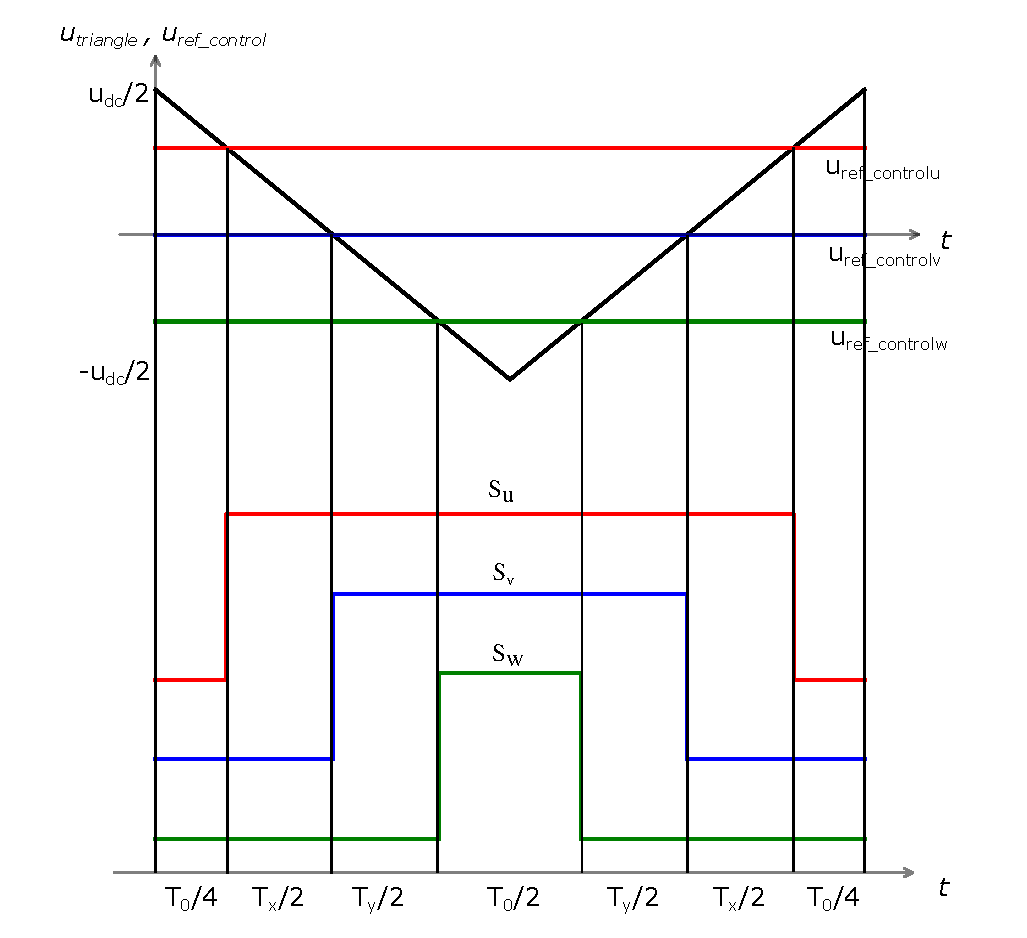
\includegraphics[width = .55\linewidth ]{svpwm_modulation_wave.pdf}
  \caption{通过载波比较的方法生成SVPWM信号}
  \label{fig:svpwm-wave}
\end{figure}

要实现对开关导通与关断的有效控制,仅仅得到矢量作用时间是不够的,还需要根据矢量作用时间计算出每个开关导通和关断的具体时刻。一个可行的方法是利用三角波与参考值进行比较,类似于对称规则采样的SPWM。如图\ref{fig:svpwm-wave}所示,采用七段式开关模式,可以保证每个开关周期内每个开关只开通关断一次。以第一扇区为例,$u_{ref\_controlu}$为A相参考波,$u_{ref\_controlv}$为B相参考波,$u_{ref\_controlw}$为C相参考波,$ T_x $为矢量$ \vec V(100) $作用时间,$ T_y $为矢量$ \vec V(110) $作用时间。根据几何关系,可以计算出这一扇区内用来与三角载波比较的参考信号$u_{ref\_controlu}$、$u_{ref\_controlv}$和$u_{ref\_controlw}$的大小。如公式2.4所示。

\begin{equation}
  \begin{aligned}
  	&u_{ref\_controlu} = \frac{U_D}{2}\frac{T_x+T_y}{T_Z}\\
  	&u_{ref\_controlv} = \frac{U_D}{2}\frac{T_y-T_x}{T_Z} \\
  	&u_{ref\_controlw} = -\frac{U_D}{2}\frac{T_x+T_y}{T_Z}
  \end{aligned}
\end{equation}

在其他扇区,参考波的计算公式与第一扇区的情况类似,只是$u_{ref\_controlu}$、$u_{ref\_controlv}$,$u_{ref\_controlw}$将分别分配给不同相,其中$u_{ref\_controlu}$分配给输出占空比最大的相,$u_{ref\_controlw}$分配给输出占空比最小的相。具体分配情况见表\ref{tab:section-referwave}。同时,$ T_x $、$ T_y $分别代表先出现的矢量和后出现的矢量的作用时间,所以需要对$ T_x $、$ T_y $的表达式进行修正,各扇区先后作用矢量时间分别对应的计算式如表\ref{tab:section-TxTy}所示。

\begin{table}[hbt]
  \centering
  \small
  \caption{各扇区SVPWM 参考波三相与实际三相对应情况}
  \label{tab:section-referwave}
  \begin{tabular}{@{}lllllll@{}}
  \toprule
  \multicolumn{1}{c}{\multirow{2}{*}{实际相}} & \multicolumn{6}{c}{ABC三相在不同扇区分别对应的参考信号} \\ \cmidrule(l){2-7} 
  \multicolumn{1}{c}{} & \multicolumn{1}{c}{\uppercase\expandafter{\romannumeral1}} & \multicolumn{1}{c}{\uppercase\expandafter{\romannumeral2}} & \multicolumn{1}{c}{\uppercase\expandafter{\romannumeral3}} & \multicolumn{1}{c}{\uppercase\expandafter{\romannumeral4}} & \multicolumn{1}{c}{\uppercase\expandafter{\romannumeral5}} & \multicolumn{1}{c}{\uppercase\expandafter{\romannumeral6}} \\ \midrule
  A相 & $u_{ref_\_controlu}$ & $u_{ref_\_controlv}$ & $u_{ref_\_controlw}$ & $u_{ref_\_controlw}$ & $u_{ref_\_controlv}$ & $u_{ref_\_controlu}$ \\
  B相 & $u_{ref_\_controlv}$ & $u_{ref_\_controlu}$ & $u_{ref_\_controlu}$ & $u_{ref_\_controlv}$ & $u_{ref_\_controlw}$ & $u_{ref_\_controlw}$ \\
  C相 & $u_{ref_\_controlw}$ & $u_{ref_\_controlw}$ & $u_{ref_\_controlv}$ & $u_{ref_\_controlu}$ & $u_{ref_\_controlu}$ & $u_{ref_\_controlv}$ \\ \bottomrule
  \end{tabular}
\end{table}


\begin{table}[hbt]
\centering
\caption{各扇区先后作用矢量时间计算式}
\label{tab:section-TxTy}
\begin{tabular}{@{}lllllll@{}}
\toprule
\multicolumn{1}{c}{\multirow{2}{*}{矢量作用时间}} & \multicolumn{6}{c}{先后作用矢量在各扇区分别对应的时间计算式} \\ \cmidrule(l){2-7} 
\multicolumn{1}{c}{} & \multicolumn{1}{c}{\uppercase\expandafter{\romannumeral1}} & \multicolumn{1}{c}{\uppercase\expandafter{\romannumeral2}} & \multicolumn{1}{c}{\uppercase\expandafter{\romannumeral3}} & \multicolumn{1}{c}{\uppercase\expandafter{\romannumeral4}} & \multicolumn{1}{c}{\uppercase\expandafter{\romannumeral5}} & \multicolumn{1}{c}{\uppercase\expandafter{\romannumeral6}} \\ \midrule
$T_x$ & $ \quad T_1 \quad$ & $ \quad T_2 \quad$ & $ \quad T_1 \quad$ & $ \quad T_2 \quad$ & $ \quad T_1 \quad$ & $ \quad T_2 \quad$ \\
$T_y$ & $ \quad T_2 \quad$ & $ \quad T_1 \quad$ & $ \quad T_2 \quad$ & $ \quad T_1 \quad$ & $ \quad T_2 \quad$ & $ \quad T_1 \quad$
\end{tabular}
\end{table}

经过上述的三个步骤,就实现了通过SVPWM的方法控制输出三相对称正弦电压信号。

\section{SVPWM参考波的数学表达}
上一节的分析已经指出,SVPWM可以通过载波比较的方法实现。那么SVPWM的载波的数学表达究竟是怎样的呢?

下面将推导采用SVPWM参考波的解析式。上一节的内容考虑的是$T_0$平均分给$\vec V(000)$和$\vec V(111)$的情况,下面将考虑更一般的情况,记$\vec V(000)$和$\vec V(111)$作用的时间分别为$T_{00}=kT_0$,$T_{07}=(1-k)T_0$。重写公式\ref{eq:T1}-\ref{eq:T2}:
\begin{equation}
  \begin{aligned}
&T_{1}=2\sqrt{3} M T_{Z} \sin \left(60^{\circ}-\theta\right)\\
&T_{2}=2\sqrt{3} M T_{Z} \sin (\theta)\\
&T_0 = T_Z - T_1 -T_2,\quad (T_{00}=kT_0,T_{07}=(1-k)T_0)
\end{aligned}
\end{equation}
其中M为调制比,它等于参考电压与直流母线电压一半的比值,$ \theta $为参考矢量与其右侧相邻矢量的夹角,$ 0\leq k\leq 1 $。参考图\ref{fig:svpwm-wave0},三相参考波表达式分别为:
\begin{equation}
  \begin{aligned}
  	&u_{u} = 1-2k+2k\frac{T_x+T_y}{T_Z}\\
  	&u_{v} = 1-2k+2k\frac{T_x+T_y}{T_Z}-\frac{2T_x}{T_Z} \\
  	&u_{w} = 1-2k+(2k-2)\frac{T_x+T_y}{T_Z}
  \end{aligned}
\end{equation}
其中$u_{u}$为输出占空比最大的相的参考波,$u_{w}$为输出占空比最小的相的参考波。同时,$ T_x $、$ T_y $分别代表先出现的矢量和后出现的矢量的作用时间。

\begin{figure}[hbt]
  \centering
  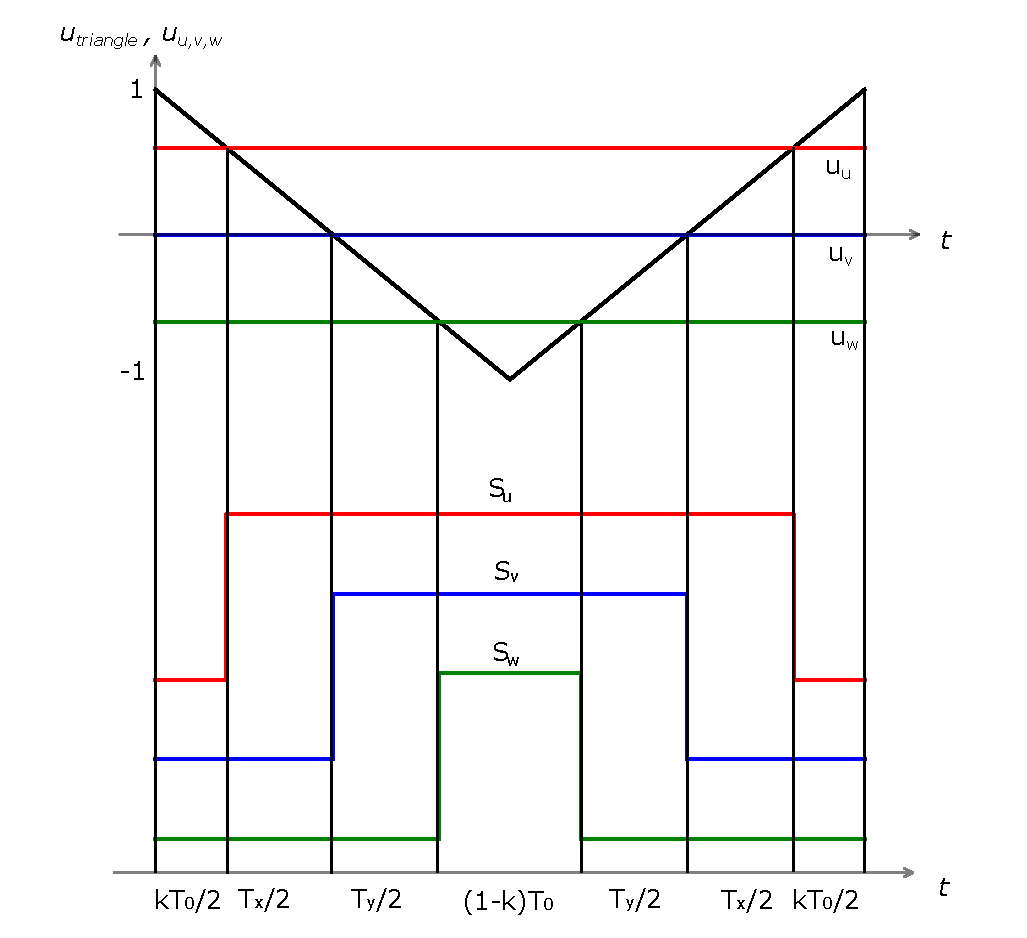
\includegraphics[width = .6\linewidth ]{svpwm_modulation_wave2}
  \caption{一般情况下SVPWM参考波与载波比较}
  \label{fig:svpwm-wave0}
\end{figure}

因为$uvw$三相对称,所以只能在基波中叠加进零序分量,否则输出的将不再是三相对称的正弦信号\footnote{更严谨的论证待补充。另外合成参考空间矢量时,两个零矢量的作用仅仅是补齐一个时间周期,而这两个零矢量产生的输出总是三相相等的,也就是说零矢量为三相对称正弦波形中注入了共模/零序分量。},可将三相参考波表示为:
\begin{equation}
   \begin{aligned}
  	&u_{ra} = u_{a} + u_z\\
  	&u_{rb} = u_{b} + u_z\\
  	&u_{rc} = u_{c} + u_z
  \end{aligned}
\end{equation}

\begin{equation}
\begin{aligned}
	u_z &= \frac{1}{3}(u_{ra}+u_{rb}+u_{rc})\\
	&= \frac{1}{3}(u_{u}+u_{v}+u_{w})\\
	&= 1-2k+2k\frac{T_x+T_y}{T_Z} - \frac{2}{3}\frac{2T_x+T_y}{T_Z}
\end{aligned}
\end{equation}
所以三相正序参考波为:
\begin{equation}
 \begin{aligned}
 	&u_1 = u_u - u_z = \frac{2}{3}\frac{2T_x+T_y}{T_Z}\\
 	&u_2 = u_v - u_z = \frac{2}{3}\frac{T_y-T_x}{T_Z}\\
 	&u_3 = u_w - u_z = -\frac{2}{3}\frac{T_x+2T_y}{T_Z}
 \end{aligned}
\end{equation}
$ u_1 $、$ u_2 $、$ u_3 $分别表示$ u_a $、$ u_b $、$ u_c $中的最大值、第二大值和最小值。将三相正序参考波相加可得$u_1 + u_2 + u_3 =0$,验证前面SVPWM的参考波是在基波中加入零序分量的假设正确。

记一步改写可得:
\begin{equation}
\begin{aligned}
	u_z &= 1-2k + k(u_1-u_3)-u_1\\
	&=1-2k-ku_3-(1-k)u_1
\end{aligned}
\end{equation}

设$u_a = M\sin(\omega t)$、$u_b = M\sin(\omega t-\ang{120})$、$u_a = M\sin(\omega t + \ang{120})$,绘制出不同$ k $取值时的参考波形,如图\ref{fig:svpwm-wave-k1}-\ref{fig:svpwm-wave-k0}所示。$ k=1/2 $时即是对称七段开关模式下的情况,$ k=1 $和$ k=0 $时有较长时间内开关没有动作,可以降低器件开关次数和开关损耗。



\begin{figure}[hbt]
  \centering
  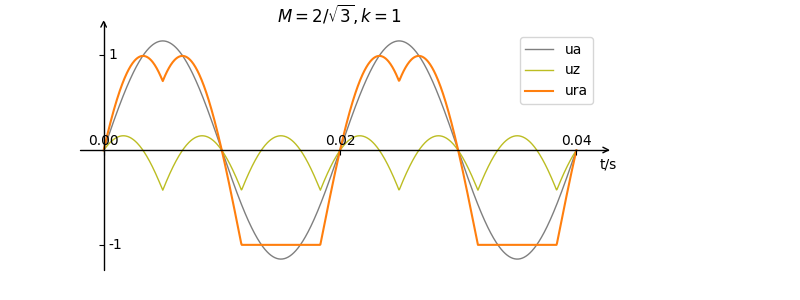
\includegraphics[width = .8\linewidth ]{svpwm_modulation_wave_k1.png}
  \caption{k=1时SVPWM参考波形}
  \label{fig:svpwm-wave-k1}
\end{figure}
\begin{figure}[hbt]
  \centering
  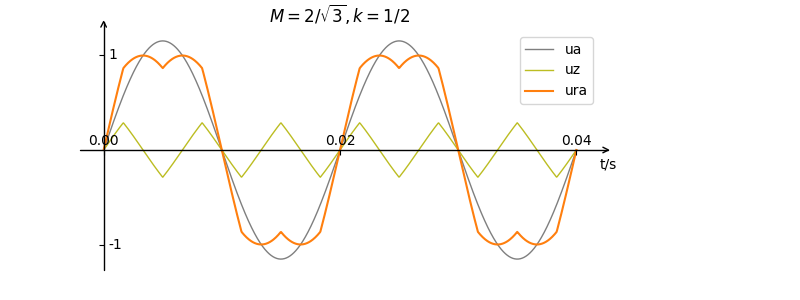
\includegraphics[width = .8\linewidth ]{svpwm_modulation_wave_k05.png}
  \caption{k=0.5时SVPWM参考波形}
  \label{fig:svpwm-wave-k05}
\end{figure}

\begin{figure}[hbt]
  \centering
  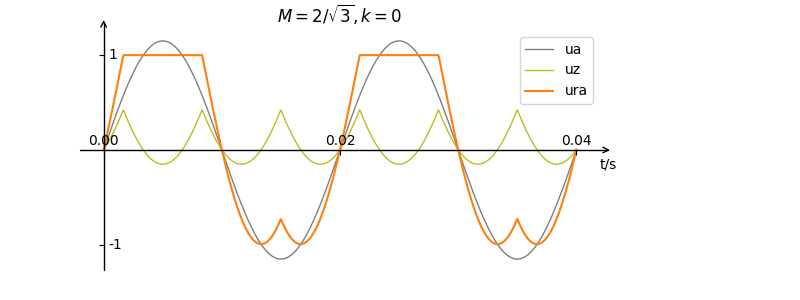
\includegraphics[width = .8\linewidth ]{svpwm_modulation_wave_k0.png}
  \caption{k=0时SVPWM参考波形}
  \label{fig:svpwm-wave-k0}
\end{figure}


\end{document}